
\chapter{frustum}
\fancyhead[RO]{\bfseries frustum}

Come abbiamo già detto, le applicazioni grafiche eseguono una serie di operazioni e trasformazioni, chiamata pipeline grafica per renderizzare una scena prelevata da un mondo virtuale 3D così come noi la vediamo a schermo. Nella figura \ref{pipeline} sono presenti le principali fasi della pipeline.

\begin{figure}[htbp]
\centering
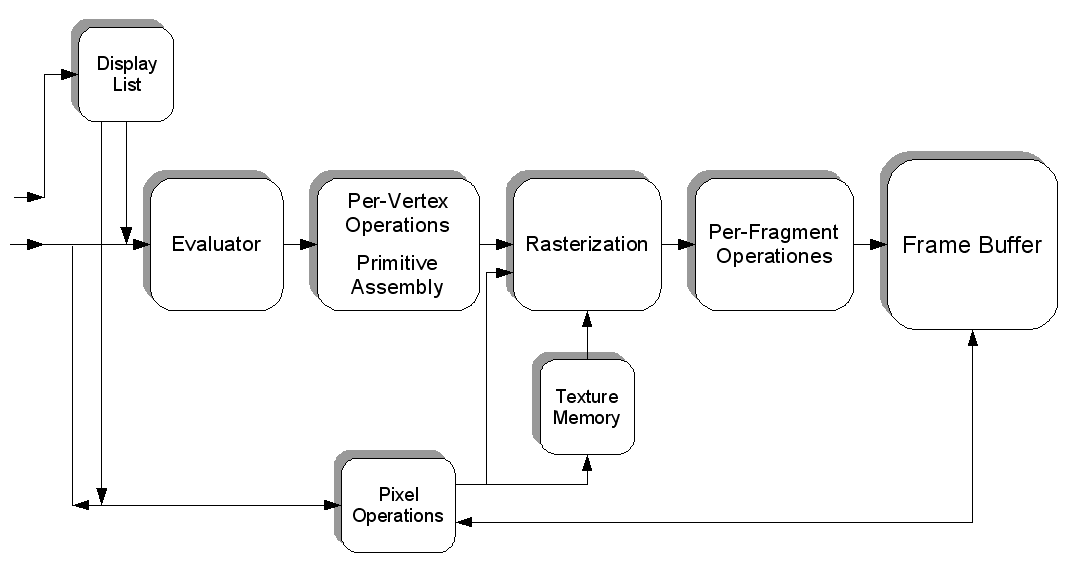
\includegraphics[width=0.7\textwidth]{images/frustum/opengl-pipeline.png}
\caption{La pipeline grafica.\label{pipeline}}
\end{figure}

Ai fini di questo progetto, ci concentreremo sulle trasformazioni, più che su altre operazioni come la rasterizzazione (conversione da vettori a pixel, costruendo segmenti o porzioni di piano che riempiono lo spazio definito da due o più vertici) o l'applicazione di materiali e texture.

\section{Le trasformazioni}
Il diagramma in figura \ref{trans-pipe} mostra le principali trasformazioni eseguite nella pipeline.

\begin{figure}[htbp]
\centering
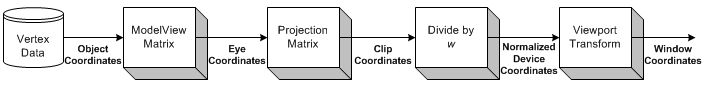
\includegraphics[width=0.7\textwidth]{images/frustum/transform-pipeline.png}
\caption{Le trasformazioni.\label{trans-pipe}}
\end{figure}

Per determinare la posizione di ciascun vertice all'interno del mondo virtuale, viene adottato un sistema di coordinate a 3 dimensioni (figura \ref{cartesian}).
\begin{figure}[htbp]
\centering
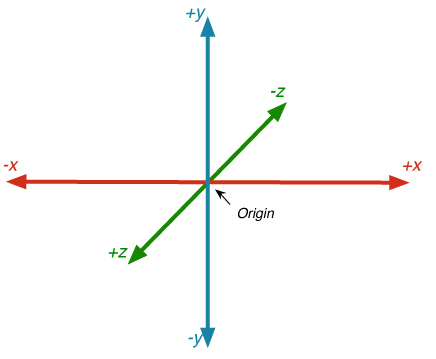
\includegraphics[width=0.3\textwidth]{images/frustum/cartesian.png}
\caption{Il sistema cartesiano in OpenGL e Ogre3D.\label{cartesian}}
\end{figure}

Da notare l'asse Z, la cui direzione positiva è quella uscente, ovvero quella rivolta verso l'utente che sta di fronte allo schermo. Questa caratteristica è fondamentale perchè determina il segno di alcuni elementi nel processo di trasformazione.

\subsection{ModelView Matrix}
Nel prima fase si utilizza una matrice chiamata Modelview Matrix, che trasforma le coordinate locali degli oggetti presenti nella scena nel sistema globale di coordinate relativo al mondo virtuale. Di default, la telecamera virtuale che inquadra la scena è posizionata nell'origine del sistema, ovvero nel punto $(0,0,0)$. La telecamera punta lo sguardo verso l'asse -Z, mentre gli assi X e Y sono paralleli al piano che rappresenta lo schermo (figura \ref{cam-default}).

\begin{figure}[htbp]
\centering
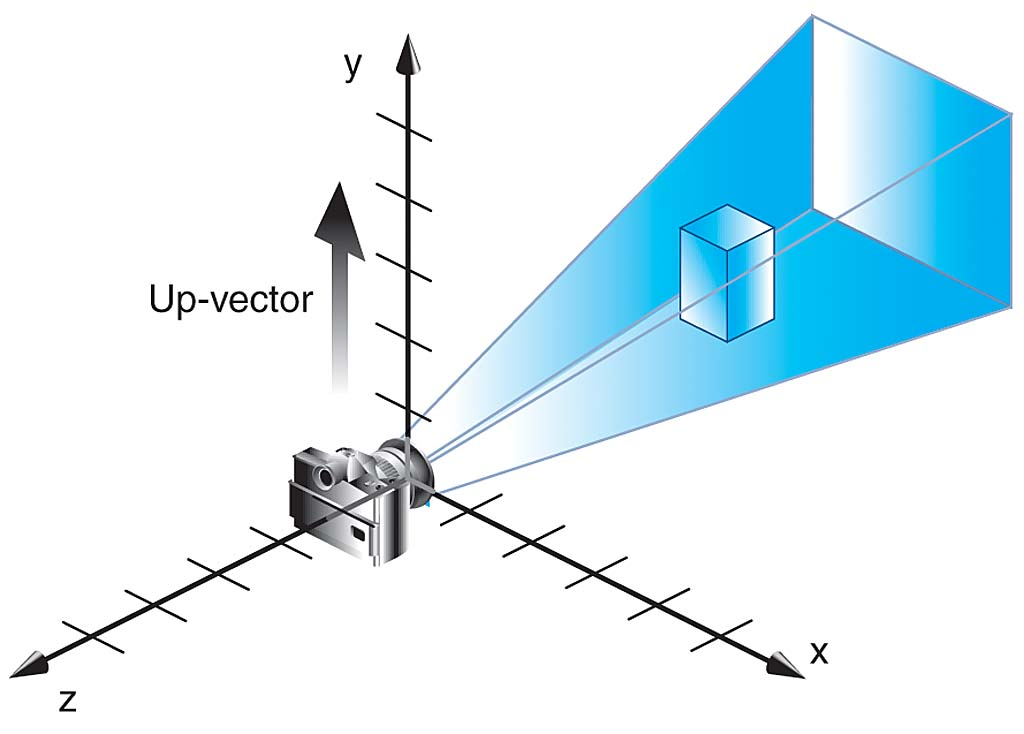
\includegraphics[width=0.5\textwidth]{images/frustum/camera-default.jpg}
\caption{La posizione di default della telecamera virtuale.\label{cam-default}}
\end{figure}


\subsection{Projection Matrix}
Lo spazio che identifica la porzione del mondo che è possibile osservare, è chiamato view volume (figura \ref{view-frustum}); tutto ciò che si trova all'interno di esso viene renderizzato nella scena.

\begin{figure}[htbp]
\centering
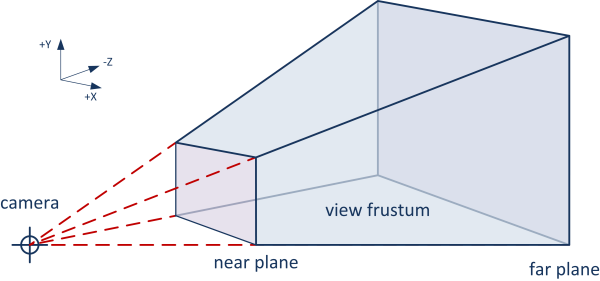
\includegraphics[width=0.5\textwidth]{images/frustum/view_frustum.png}
\caption{Il view volume nella proiezione prospettica.\label{view-frustum}}
\end{figure}

Questo spazio è caratterizzato da un piano più vicino alla telecamera, il near plane, e uno più lontano, il far plane. Il near plane rappresenta la coordinata Z dalla quale sarà renderizzata la scena, ovvero tutto ciò che sta dietro non sarà visibile. Il far plane rappresenta la coordinata Z di fine scena, perciò determina quanto in profondità essa è visibile.

La Projection Matrix ha il compito di trasformare il view volume in un cubo $2 \times 2\times 2$ centrato nell'origine, determinando anche la trasformazione di tutto ciò che è presente al suo interno. Ogni vertice all'interno di esso avrà coordinate $-1\leq x,y,z \leq 1$.

Il modo in cui viene considerato il view volume, e quindi il modo in cui viene trasformato lo spazio, dipende dal tipo di proiezione. Essenzialmente esistono due tipi di proiezione, quella ortogonale e quella prospettica.

\begin{figure}[htbp]
\centering
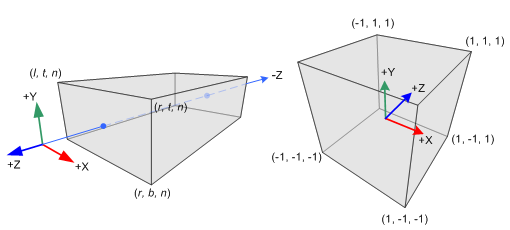
\includegraphics[width=0.5\textwidth]{images/frustum/orto-projection.png}
\caption{Trasformazione con proiezione ortogonale.\label{orto}}
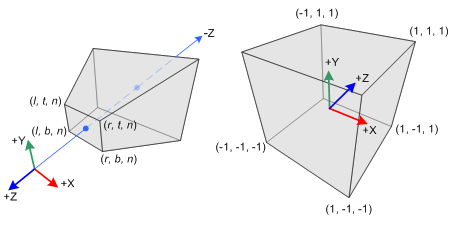
\includegraphics[width=0.5\textwidth]{images/frustum/persp-projection.png}
\caption{Trasformazione con proiezione prospettica.\label{persp}}
\end{figure}

In quella ortogonale (figura \ref{orto}) il view volume è rappresentato da un parallelepipedo; in questo caso tutti i vertici vengono proiettati sul near plane, parallelamente alla direzione della telecamera. Il risultato sarà quello di avere una visione non prospettica della scena.

La proiezione prospettica (che vedremo in dettaglio in seguito, in quanto il suo uso è fondamentale in questo progetto) presenta un view volume che ha la forma di un tronco di piramide, in inglese frustum.
Il vertice della piramide è dato dalla posizione della telecamera, mentre il near plane e il far plane sono rispettivamente la base minore e maggiore del frustum. In questo caso i vertici vengono proiettati sul near plane seguendo la direzione che li congiunge alla telecamera. Dopo aver applicato questa trasformazione, il frustum diventerà un cubo, e tutti gli oggetti al suo interno saranno deformati per come sono visti a schermo.

Nelle figure \ref{example1} e \ref{example2} è possibile vedere un esempio di questa trasformazione.
\begin{figure}[htbp]
\centering
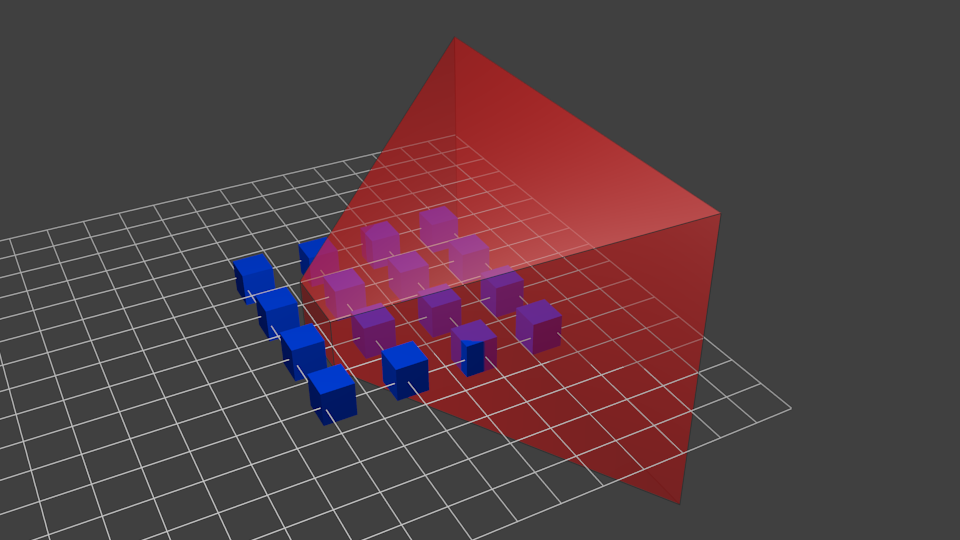
\includegraphics[width=0.6\textwidth]{images/frustum/frustum_cubes.png}
\caption{Il frustum prima della trasformazione.\label{example1}}
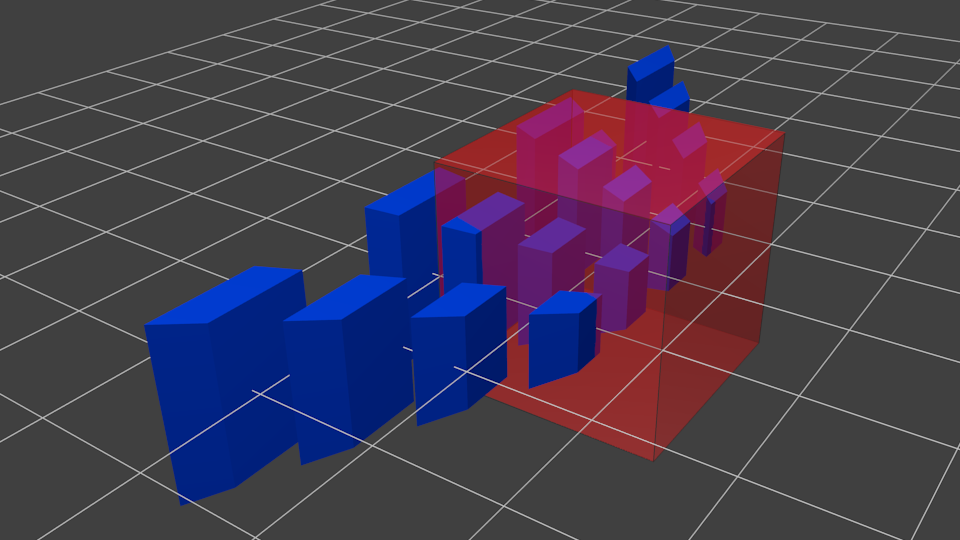
\includegraphics[width=0.6\textwidth]{images/frustum/frustum_homogeneous.png}
\caption{Il frustum trasformato nel sistema di coordinate omogeneo.\label{example2}}
\end{figure}

Nella figura \ref{example3} il cubo è visto dal suo piano frontale.

\begin{figure}[htbp]
\centering
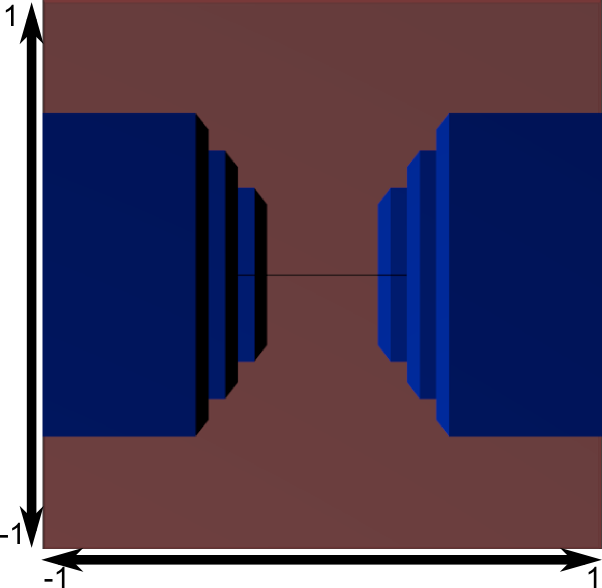
\includegraphics[width=0.5\textwidth]{images/frustum/frustum_view.png}
\caption{Il nuovo frustum visto in prospettiva.\label{example3}}
\end{figure}

Nella projection matrix è compresa l'operazione che normalizza i vertici, mappando le coordinate in modo che siano comprese tra $-1$ e $1$. Questa normalizzazione è data da una divisione delle componenti di ogni vertice per la quarta componente, cioè la coordinata W.


L'utilizzo della quarta coordinata per definire i vertici dà origine al sistema di coordinate omogenee. Questo sistema, introdotto da August Ferdinand Möbius intorno al 1837, prevede la rappresentazione di $N$ coordinate con vettori di $N+1$ dimensioni, ed è usato per descrivere i punti nella geometria proiettiva. Inoltre la quarta coordinata permette di rappresentare tutte le trasformazioni affini (trasformazioni lineari più una traslazione) tramite le matrici.

Considerando che la traslazione di un vettore a due dimensioni $v = (x,y)$ per un vettore $v_0 = (a,b)$
è data dalla loro somma, è possibile rappresentare questa trasformazione anche tramite una matrice $3\times3$:
$$T_{v_0} \times v = \begin{pmatrix} 1 & 0 & a \\
0 & 1 & b \\
0 & 0 & 1
\end{pmatrix}
\begin{pmatrix}
x \\
y \\
1 
\end{pmatrix}
=
\begin{pmatrix}
x + a \\
y + b \\
1
\end{pmatrix}$$\\

E' possibile estendere questo concetto ad ogni tipo di trasformazione, permettendo di raggruppare più trasformazioni in una singola matrice uguale al prodotto delle matrici che le rappresentano.

\subsection{Viewport Matrix}
L'ultimo passaggio è dato dalla Viewport Matrix, che trasforma i vertici in coordinate relative allo schermo. Dopo questa fase, il nuovo sistema di riferimento è relativo all'angolo in basso a sinistra della finestra aperta dopo aver lanciato l'applicazione, e le coordinate sono date dai pixel dello schermo.

Dati i valori \textit{w} (width = larghezza) e \textit{h} (height = altezza), in pixel, il canonical view volume viene ridotto, scalandolo di $w/2$ nella direzione orizzontale e di $h/2$ nella direzione verticale. Dopo di ciò il tutto viene traslato di un vettore $(-w/2, -h/2, -1)$ per allineare l'angolo in basso a sinistra di fronte del canonical view volume (cioè il punto $(-1,-1,-1)$) con l'angolo in basso a sinistra della finestra visualizzata a schermo.

Tutte le operazione che si svolgono dopo, come la rasterizzazione e lo shading, vengono fatte usando questo sistema di riferimento.

\section{La teoria matematica delle trasformazioni}

\subsection{Il view frustum}
Con view frustum indichiamo il view volume utilizzato nella proiezione prospettica, in quanto il frustum rappresenta il tronco di piramide che racchiude lo spazio visibile del mondo 3D; in genere viene chiamato allo stesso modo anche il view volume considerato nella proiezione ortogonale, ma in questo caso occorre notare che si tratta di un parallelepipedo e non un tronco di piramide.

Il view frustum è posizionato in modo che il vertice della piramide, rappresentante l'osservatore o la telecamera, giaccia sull'origine. Esso è composto da sei piani, due di questi li abbiamo già visti, e sono il near e il far plane. Gli altri quattro rappresentano le coordinate che definiscono i bordi del near plane, e sono chiamati left, right, bottom e top planes.


\begin{figure}[htbp]
\centering
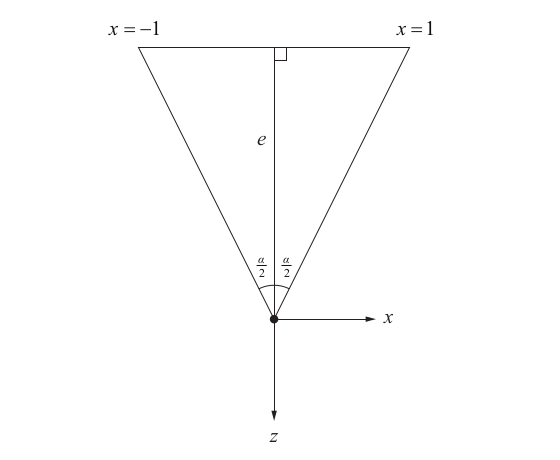
\includegraphics[width=0.6\textwidth]{images/frustum/frustum-x.png}
\caption{La distanza focale $e$ dipende dall'angolo dell'apertura $\alpha$ della telecamera. \label{frustum-x}}
\end{figure}

Si considera, in generale, che il piano di proiezione sia situato ad una distanza $e$ dall'osservatore, in modo che le coordinate del left e right plane siano rispettivamente $x=-1$ e $x=+1$ (figura \ref{frustum-x}).

La distanza $e$ è la distanza focale, che è determinata dall'angolo di apertura $\alpha$ della telecamera: valori più alti di $\alpha$ determinano valori di $e$ più piccoli, e ciò si traduce in un accorciamento della distanza e allargamento della visuale, creando un effetto grandangolare, in quanto il piano di proiezione è piu vicino all'osservatore; viceversa valori alti di $e$ determinano un allontanamento del piano di proiezione, con effetto di allungamento della distanza e restringimento della visuale.

Grazie alla trigonometria possiamo calcolare la distanza focale a partire dall'angolo di apertura, come  $$e = \frac{1}{\tan(\alpha/2)}$$.

Un altro valore da tenere in considerazione è l'aspect ratio , cioè il rapporto tra la lunghezza e l'altezza del piano. Per esempio in uno schermo $1920\times 1080$ l'aspect ratio è uguale $\frac{1080}{1920}=\frac{16}{9}$, oppure in uno schermo $640\times 480$ è $\frac{640}{480}=\frac{4}{3}$.Grazie a questo possiamo determinare il formato della finestra che vogliamo visualizzare a schermo.

\begin{figure}[htbp]
\centering
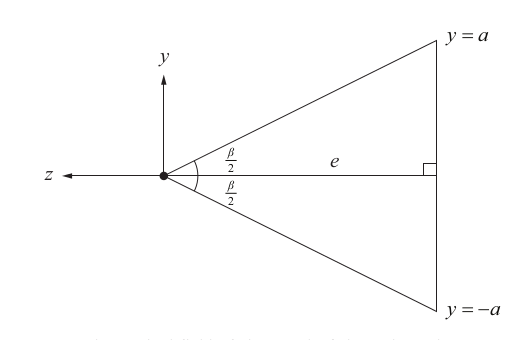
\includegraphics[width=0.6\textwidth]{images/frustum/frustum-y.png}
\caption{L'angolo di apertura verticale $\beta$ dipende dall'aspect ratio.\label{frustum-y}}
\end{figure}

Considerando che il left e right plane hanno coordinate $x=-1$ e $x=+1$, il bottom e top plane vengono posizionati alle coordinate $y=-a$ e $y=+a$, dove $a$ è il reciproco dell'aspect ratio; nel caso $\frac{16}{9} \rightarrow a=\frac{9}{16}=0.5625$ (figura \ref{frustum-y}).

Possiamo calcolare l'angolo di apertura verticale $\beta$ come: $$\beta=2\tan^{-1}(a/e)$$ 

Possiamo assegnare arbitrariamente un valore $n$ come coordinata per il near plane, in modo da determinare la distanza da cui inizia il frustum. Le coordinate dei quattro piani ora devono essere ricalcolate come $$x =\pm \frac{n}{e}$$ e $$y = \pm \frac{an}{e}$$.



\subsection{Projection Matrix}
Come abbiamo detto all'inizio del capitolo, per renderizzare a schermo un punto tridimensionale, esso deve essere trasformato in un punto a due dimensioni. Il sistema di coordinate omogenee,  che si utilizza per identificare i punti nello spazio, possiede quattro dimensioni. La projection matrix lo trasforma in un sistema a tre dimensioni, proiettando lo spazio omogeneo in uno spazio 3D chiamato canonical view volume (un cubo).

Dopo aver proiettato i punti omogenei sul near plane, le nuove coordinate vengono normalizzate, cioè divise per la quarta coordinata $w$; questo permette di mappare le nuove coordinate in uno spazio $[-1,1]$.

Consideriamo un punto omogeneo $P=\langle P_x,P_y,P_z,1\rangle$ situato nel view frustum.
Riprendendo il discorso del paragrafo precedente riguardante i triangoli simili,  le coordinate $x$ e $y$ del punto proiettato sul near plane sono
\begin{center}
$x=-\frac{n}{P_z}{P_x}$ \,\,\,e\,\,\,  $y=-\frac{n}{P_z}{P_y}$
\end{center}
$$\begin{array}{cc}
x=-\frac{n}{P_z}{P_x} & y=-\frac{n}{P_z}{P_y}\\
\end{array}$$\\


Allora $l\leq x\leq r$ e $b\leq y\leq t$, dove l,r,b,t sono le coordinate dei quattro piani del frustum, descritti in precedenza.
Per mappare le nuove coordinate x e y si usano le funzioni lineari:
$$x'=(x-l)\frac{2}{r-l}-1$$ e $$y'=(y-b)\frac{2}{t-b}-1$$
Sostituendo alla x e alla y le espressioni scritte in precedenza e semplificando otteniamo:
$$x'=\frac{2n}{r-l}\left(-\frac{P_x}{P_z}\right)-\frac{r+l}{r-l}$$ e 
$$y'=\frac{2n}{t-b}\left(-\frac{P_y}{P_z}\right)-\frac{t+b}{t-b}$$\\
Per quanto riguarda la mappatura della coordinata z, si deve trovare una funzione che porti $-n\rightarrow -1$ e $-f\rightarrow 1$.
Considerando che le coordinate z hanno i reciproci interpolati, possiamo scrivere una funzione di $1/z$:
$$z'=\frac{A}{z}+B$$
Abbiamo detto che $-n\rightarrow -1$ e $-f\rightarrow 1$, perciò possiamo ottenere il sistema:
$$-1=\frac{A}{-n}+B$$ e $$1=\frac{A}{-f}+B$$
Risolvendo il sistema otteniamo:
$$A=\frac{2nf}{f-n}$$ e $$B=\frac{f+n}{f-n}$$\\
Sostituendo $A$ e $B$:
$$z'=-\frac{2nf}{f-n}\left(-\frac{1}{P_z}\right)+\frac{f+n}{f-n}$$
Si può notare che nelle equazioni di $x'$, $y'$ e $z'$ è presente una divisione per $-P_z$: il punto tridimensionale $P'=\langle x',y',z'\rangle$ è equivalente al punto omogeneo 4D $P=\langle -x'P_z,-y'P_z,-z'P_z,-P_z\rangle$ dopo che esso viene diviso per la sua coordinata w, cioè per $-P_z$.
Perciò possiamo esprimere le precedenti equazioni mettendo in evidenza $-x'P_z$, $-y'P_z$, e $-z'P_z$:
$$-x'P_z=\frac{2n}{r-l}P_x+\frac{r+l}{r-l}P_z$$, 
$$-y'P_z=\frac{2n}{t-b}P_y+\frac{t+b}{t-b}P_z$$e
$$-z'P_z=-\frac{f+n}{f-n}P_z-\frac{2nf}{f-n}$$

Essendo funzioni lineari delle coordinate del punto $P$, possiamo utilizzare una matrice $4\times 4$ per rappresentare la trasformazione prospettiva; moltiplicando la matrice per il punto P, otteniamo la sua proiezione $P'$ sul near plane:
$$P'=M*P=
\begin{bmatrix}
\frac{2n}{r-l} & 0 & \frac{r+l}{r-l} & 0 \\
0 & \frac{2n}{t-b} & \frac{t+b}{t-b} & 0 \\
0 & 0 & -\frac{f+n}{f-n} & -\frac{2nf}{f-n} \\
0 & 0 & -1 & 0
\end{bmatrix}
\begin{bmatrix}
P_x \\ P_y \\ P_z \\ 1
\end{bmatrix}$$

In OpenGL esistono essenzialmente due funzioni per generare una matrice di proiezione prospettica: la libreria GLM (OpenGL Mathematics), usata in questo progetto (nella versione sviluppata in OpenGL), offre i metodi \texttt{perspective(float fov, float aspect, float n, float f)}
e \texttt{glFrustum(float l,float r,float t,float b,float n,float f)}.

La prima funzione restituisce una matrice di proiezione con frustum simmetrico, ovvero il near plane assume la figura di un rettangolo; questo è il tipo di frustum maggiormente utilizzato; come visto all'inizio del paragrafo relativo al view frustum, tramite l'angolo di apertura di campo fov, e l'aspect ratio, è possibile calcolare le coordinate dei quattro piani del frustum, oltre al near e il far. Dopo aver calcolato le coordinate, la funzione genera la matrice desiderata.

La seconda funzione invece prende in input le coordinate dei sei piani del frustum e calcola direttamente la matrice; in questo modo è anche possibile creare un frustum asimmetrico, generando una prospettiva distorta (il near plane può assumere la forma di un quadrilatero qualsiasi).

Quest'ultima funzione è stata utilizzata in questo progetto, in modo da avere la possibilità di distorcere la prospettiva della scena in base alla posizione dell'osservatore.  

\subsection{View Matrix}
La Projection Matrix trasforma lo spazio considerando che la telecamera sia situata nell'origine e che la direzione dello sguardo sia rivolto lungo l'asse negativo delle Z. Per questo, se la telecamera è posizionata in punti diversi, si deve applicare un'altra trasformazione, che porti la telecamera nella sua posizione di default. Questa trasformazione è data dalla View Matrix, che ha il compito di trasformare lo spazio di coordinate del mondo 3D nello spazio di coordinate relativo alla telecamera. In pratica la telecamera viene ruotata e traslata per essere posizionata nell'origine, con il corretto orientamento, e nello stesso momento tutto il mondo 3D subisce la stessa trasformazione (figure \ref{view1} e \ref{view2}).

\begin{figure}[htbp]
\centering
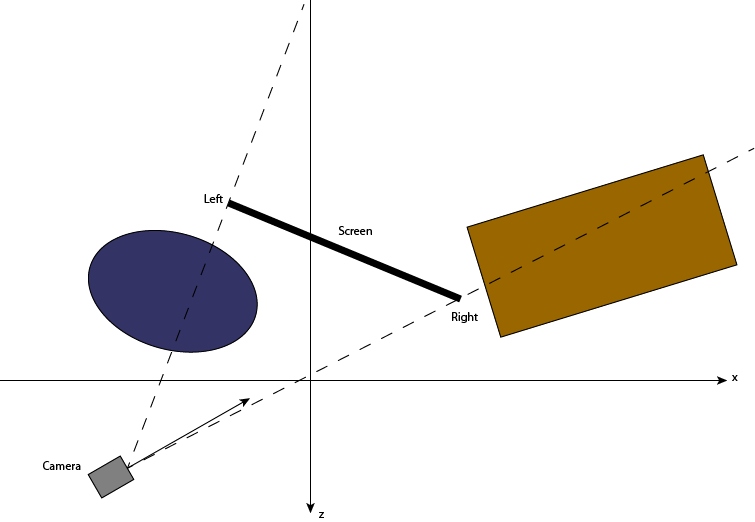
\includegraphics[width=0.5\textwidth]{images/frustum/view-matrix1.png}
\caption{Una scena con la telecamera posta in un punto qualsiasi.\label{view1}}
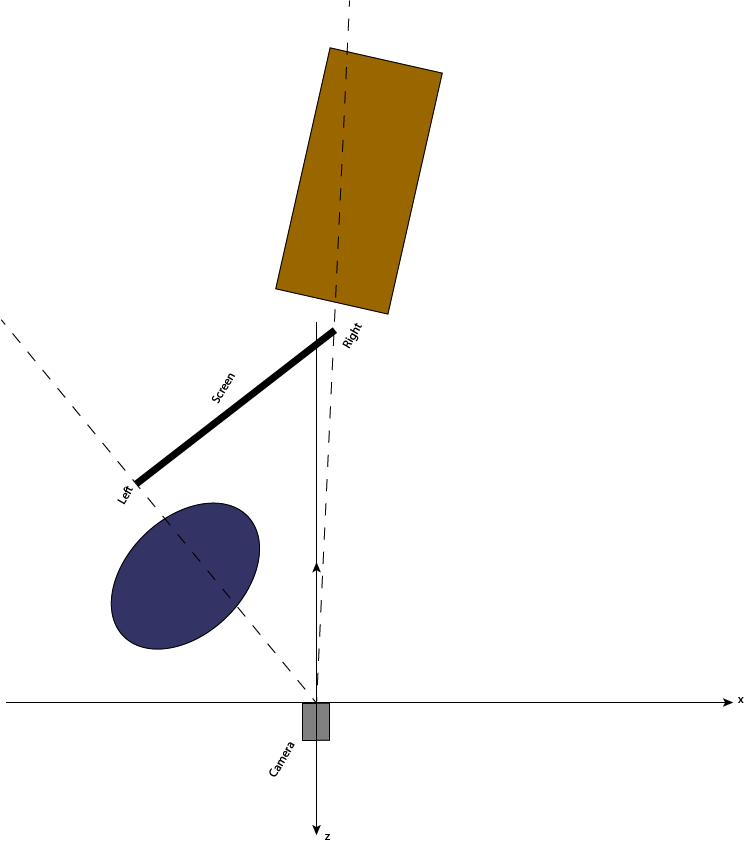
\includegraphics[width=0.5\textwidth]{images/frustum/view-matrix2.png}
\caption{La scena trasformata con la view matrix.\label{view2}}
\end{figure}


Dopo aver applicato questa trasformazione è possibile applicare anche la proiezione.

Il calcolo della view matrix necessita di tre vettori:
\begin{itemize}
\item \textbf{eye}: identifica la posizione della telecamera.
\item \textbf{target}: identifica il punto verso cui è rivolto lo sguardo.
\item \textbf{up}: identifica la direzione che punta verso l'alto, di solito coindice con l'asse y, quindi è $(0, 1, 0)$.
\end{itemize}

La matrice consiste in due trasformazioni: una rotazione, per allineare l'orientamento della telecamera con l'asse negativo delle Z, e una traslazione, per spostare la telecamera nell'origine.
Per la rotazione si calcola una base ortonormale che rappresenta il sistema di coordinate relativo alla telecamera, tramite i tre vettori, ponendo\\
$n = normalize(eye - target)$\\
$u = normalize(cross(up,n))$\\
$v = cross(n,u)$\\
dove $cross(a,b)$ rappresenta il prodotto vettoriale tra $a$ e $b$ e $normalize(a)$ la normalizzazione di $a$. I vettori u,v,n formano la base ortonormale desiderata.

La matrice che orienta la scena nel modo corretto è:
$$R=
\begin{bmatrix}
u.x && u.y && u.z && 0\\
v.x && v.y && v.z && 0\\
n.x && n.y && n.z && 0\\
0 && 0 && 0 && 1\\
\end{bmatrix}
$$

Per quanto riguarda la traslazione basta utilizzare la matrice

$$T=
\begin{bmatrix}
0 && 0 && 0 && -eye.x\\
0 && 0 && 0 && -eye.y\\
0 && 0 && 0 && -eye.z\\
0 && 0 && 0 && 1\\
\end{bmatrix}
$$\\
dove il meno permette di traslare la scena in modo che la telecamera finisca nell'origine.

La View Matrix è data dal prodotto della matrice dell'orientamento per quella di traslazione.
Possiamo perciò scriverla in modo compatto come:
$$V = R \times T =
\begin{bmatrix}
u.x && u.y && u.z && -dot( u, eye )\\
v.x && v.y && v.z && -dot( v, eye )\\
n.x && n.y && n.z && -dot( n, eye )\\
0 && 0 && 0 && 1\\
\end{bmatrix}
$$\\
dove $dot(a,b)$ rappresenta il prodotto scalare tra $a$ e $b$.


